\documentclass{article}
\usepackage{v-problem}
\vgeometry

\begin{document}
\vtitle[KINEMATICS]

\def\pn{04}
\def\book{Irodov}
\def\page{13}
\def\gdrive{https://drive.google.com/drive/folders/1THMFeX_mmLal7QTLWi865ejPslNpG_VS?usp=share_link}

\def\question{
Point $A$ moves uniformly with velocity $v$ so that the vector $\vec{v}$ is continually "aimed" at point $B$ which in its turn moves rectilinearly and uniformly with velocity $u<v$. At the initial moment of time $\vec{v} \perp \vec{u}$ and the points are separated by a distance $l$. How soon will the points converge?
}

\def\option{
}

\def\diagram{
\begin{center}
\begin{tikzpicture}
[thick]
\tzline[dashed](0, 0)(5, 0)
\tzline+[->, thick](0, 0)(1, 0){$\vec{u}$}[ar=2mm]
\tzline[dashed](0, 0)(0, -4)
\tzline[|<->|]<-0.5, 0>(0, 0)(0, -4){$l$}[l=2mm, midway]
\tzline+[->](0, -4)(0, 1){$\vec{v}$}[al=2mm]
\tzdots*<0, 0.09>(0, 0)(0, -4);(5pt)
\tzto[out=90,in=180,dashed](0,-4)(5,0)
\end{tikzpicture}
\end{center}
}

\vspace*{\fill}
\begin{tikzpicture}
	\node[qnumber] (n) at (0, 0)[scale=2] {$\pn.$};
	\node[question] (q) [right=2mm of n.east] {\question};
	\tzline[divider]<-0.125, 0> (q.north west)(q.south west);
	\node[format] (f) at  (q.south east){[\book \quad \page]};
	\node[diagram] (d) [below=1cm of q.south] {\diagram};
	\node[option] (o) [below=0.1cm of d.south] {\option};
\end{tikzpicture}	
\vspace*{\fill}

\pagebreak
\vtitle[\texttt{SOLUTION}]

\begin{center}
\begin{tikzpicture}
[thick]
\def\tangentat{0.8}
\tzline[dashed]"HL"(0, 0)(5, 0)
\tzline[dashed](0, 0)(0, -4)
\tzline[|<->|]<-0.5, 0>(0, 0)(0, -4){$l$}[l=2mm, midway]
\tzto[out=90,in=180,dashed]"path"(0,-4)(5,0)
\tztangentat[dashed, thick]"TL"{path}{\tangentat}[\tangentat:3.5]
\tztangentat[->, thick]{path}{\tangentat}[\tangentat:\tangentat + 1]{$\vec{v}$}[al]
\tzXpoint{HL}{TL}(X)
\tzline+[->](X)(1, 0){$\vec{u}$}[ar=2mm]
\tzvXpointat*{path}{\tangentat}{$A$}[above left=2mm](5pt)
\tzdot*(X)(5pt)
\tznode(X){$B$}[a=2mm]
\tzvXpointat{TL}{3}(A)
\tzanglemark(5, 0)(X)(A){$\theta$}
\end{tikzpicture}
\end{center}

At any moment distance between $A$ and $B$ is $s(AB)$ and this distance being covered by relative velocity of both these particles in the direction of $AB$. 

\begin{align}
-\dfrac{\d{s}}{\d{t}} &= v - u\cos\theta 
\end{align}

\pagebreak

As both the particles $A$ and $B$ covered the same horizontal distance so,
\begin{align}
\int_0^t u\d{t} = \int_0^t v\cos\theta\d{t}
\end{align}

From equation (1)
\begin{align*}
-\int_l^0 \d{s} &= \int_0^t \left( v -u\cos\theta \right) \d{t}\\
l &= vt - u\int_0^t \cos\theta \d{t}\\ 
\int_0^t \cos\theta \d{t} &= \dfrac{vt-l}{u}
\end{align*}

Now put this integral value in equation (2)
\begin{align*}
\int_0^t u\d{t} &= \int_0^t v\cos\theta\d{t}\\
ut &= v\int_0^t \cos\theta \d{t}\\
ut &= v \left(\dfrac{vt-l}{u}\right)\\
u^2t &= v^2t -vl \\
t &= \dfrac{vl}{v^2-u^2}\ans
\end{align*}

\pagebreak

\vspace*{\fill}
\begin{center}
	\fbox{\qrcode[height=2cm]{\gdrive}}
\end{center}
\vspace*{\fill}
\end{document}
